% According to Elsevier instructions https://www.elsevier.com/authors/policies-and-guidelines/latex-instructions
\documentclass[10pt]{elsarticle}
\usepackage{graphicx,natbib,amssymb,amsmath}

% To remove the line "Preprint submitted to Elsevier" imposed by the document class "elsarticle.cls"
\makeatletter
\def\ps@pprintTitle{%
 \let\@oddhead\@empty
 \let\@evenhead\@empty
 \def\@oddfoot{}%
 \let\@evenfoot\@oddfoot}
\makeatother

%\usepackage{nopageno}
\usepackage{upgreek}
\usepackage{enumitem} % enriched labeled item
\usepackage{array} % for using "fixed column width", see https://www.overleaf.com/learn/latex/Tables
% Define some new column types for easier horizontal alignments for fixed width columns, see https://tex.stackexchange.com/questions/12703/how-to-create-fixed-width-table-columns-with-text-raggedright-centered-raggedlef for details.
\newcolumntype{L}[1]{>{\raggedright\let\newline\\\arraybackslash\hspace{0pt}}m{#1}}
\newcolumntype{C}[1]{>{\centering\let\newline\\\arraybackslash\hspace{0pt}}m{#1}}
\newcolumntype{R}[1]{>{\raggedleft\let\newline\\\arraybackslash\hspace{0pt}}m{#1}}

\graphicspath{ {./} } % Note that paths with underscore '_' or hyphen '-' should be avoided. 
\DeclareGraphicsExtensions{.pdf,.png,.jpg}

\usepackage{hyperref} % makes the references hyperlink
\usepackage{cleveref} % uses \cref
\crefname{enumi}{eq}{eqs} % reference any "\item" with "\label{eqs:*}" as "\equation"

% set paragraph verticle spacing
\setlength{\parskip}{4.8pt}

% use the "\caption*{}" command
\usepackage{caption} 
\newcommand\fnote[1]{\captionsetup{width=.9\linewidth,font=footnotesize}\caption*{#1}}

\usepackage{mathrsfs}

\begin{document}
\begin{frontmatter} % comment out this when using "htlatex/make4ht"

\title{A Fuel-optimal Landing Guidance and Inverse Kinematics coupled PID Control Solution for Power-descent Vertical Landing in Simulation}

\author{Yongfeng Lu}
\ead{genxium@hotmail.com}
\author{Zejian Chen}
\ead{alteracfinished1111@gmail.com}
\address{Shenzhen Lokcol Interactive Ltd.}
\address{Block 8, $1^{st}$ Weiye Road, Dongguan City, Guangdong Province, China}
\maketitle

\begin{abstract}
This article presents a guidance path planning and realtime control solution for power-descent landing of an ovoid-shape vehicle in simulation. Given a vehicle initially in free-fall state at a location in mid-air site, the proposed solution will guide and control it by the thrusters to land it at a target location on the ground.         

The solution consists of an offline guidance path planning step and a realtime control step. It uses the result of a convexified guidance path planning to tune an \textit{Inverse Kinematics (IK) coupled PID controller} with feedforward routes. In a \textit{Bullet Physics}\cite{bulletphy} based simulation environment, experiments were conducted to show good alignment with guidance, i.e. averaged \textit{Root Mean Square Error (RMSE)} of position, velocity and attitude-in-quaternion are within $1.00 \, m$, $2.00 \, m/s$ and $0.10$ respectively during a divert up to $120 \, m$ horizontally and $100 \, m$ vertically, against several disturbances(e.g. reducing mass, fluctuating \textit{center of mass}, scheduling uncertainty and simulated wind), while the simulation frame rate is kept at around 60 fps for convenient realtime interaction. 
\end{abstract}

\begin{keyword}
simulation, convex optimization, path planning, SOCP, Inverse Kinematics, PID, feedforward control, robust control   
\end{keyword}
\end{frontmatter}

% set verticle spacing for consecutive "\begin{equation} ... \end{equation}"s, should put AFTER "\begin{document}"
\abovedisplayskip=3pt
\abovedisplayshortskip=3pt
\belowdisplayskip=0pt
\belowdisplayshortskip=0pt
\abovecaptionskip=0pt
\belowcaptionskip=0pt

\section{Introduction} \label{sec:intro}
Power-descent vertical landing has been of much interest in simulation of \textit{Guidance, Navigation and Control(GNC)}. For \textit{guidance} \cite{cvxpow, losslesscvx} proposed a convex programming approach for planning a fuel-optimal path as well as the accompanying control sequence for the \textit{center of mass}, which was brought to successful field test in cooperation with the vehicle and attitude controller provided by Masten Space Systems \cite{gfoldexp}. This guidance approach will be later reviewed and applied in \cref{sec:gdp} for path planning with desired constraints.   

While guidance approach takes care of path of the \textit{center of mass}, for \textit{control} an actual simulation of vehicle landing requires a \textit{control} approach that applies to a 3D object with non-zero volume and an attitude. Recent literatures showed that several popular general purpose controllers, e.g. \textit {Model Predictive Control (MPC)}\cite{wang2019optimal, botelho2022design}, \textit{Linear Quadratic Regulator (LQR)}\cite{kim2020modeling} and \textit{PID} \cite{kim2020modeling, jo2011control, hilmi2019lunar}, are all feasible in their contexts. 

Regardless of its popularity, \textit{MPC} is not often an ideal choice when it comes to a need of fast response, i.e. in millisecond timescale \cite{ferreau2011model}. Recent review\cite{schwenzer2021review} showed that in certain cases with parallelisation, iterative learning and other tailored optimisations, one can accelerate \textit{MPC} significantly, yet still involving heavy empirical tuning. The \textit{LQR control} on the otherhand, requires not only empirical tuning of the \textit{Q, R} matrices but also of linearizing the dynamics by a chosen partial-state\cite{kim2020modeling} when full-state linearization is not viable, which further complicates the design in theoretical analysis\cite{sarras2008partial}. The traditional design methodology of \textit{PID control} involves much empirical tuning for complicated dynamics as well, but can be analytical for certain simple dynamics\cite{skogestad2012simc, grimholt2016optimal, ruscio2017tuning}. 

This article proposed an \textit{IK coupled PID controller} to help the vehicle follow the guidance path, where an \textit{IK Estimator}(\cref{sec:ikestimator}) reduces the translational and attitude dynamics of interest to a simple \textit{no delay, no damp double integrating transfer function} whose PID design parameters $K_{p}$, $K_{d}$ can be analytically determined.    

The simulation environment used by this article comes with more disturbances(\cref{sec:disturbance}) than the aforementioned literatures as well, in terms of covering propellant consumption, varying \textit{center of mass} of the vehicle, multithreading uncertainty and simulated wind, which the control should be robust to while keeping a high simulation frame rate.      

\section{Problem Description} \label{sec:problem} 

\begin{figure}[htb]
    \centering
    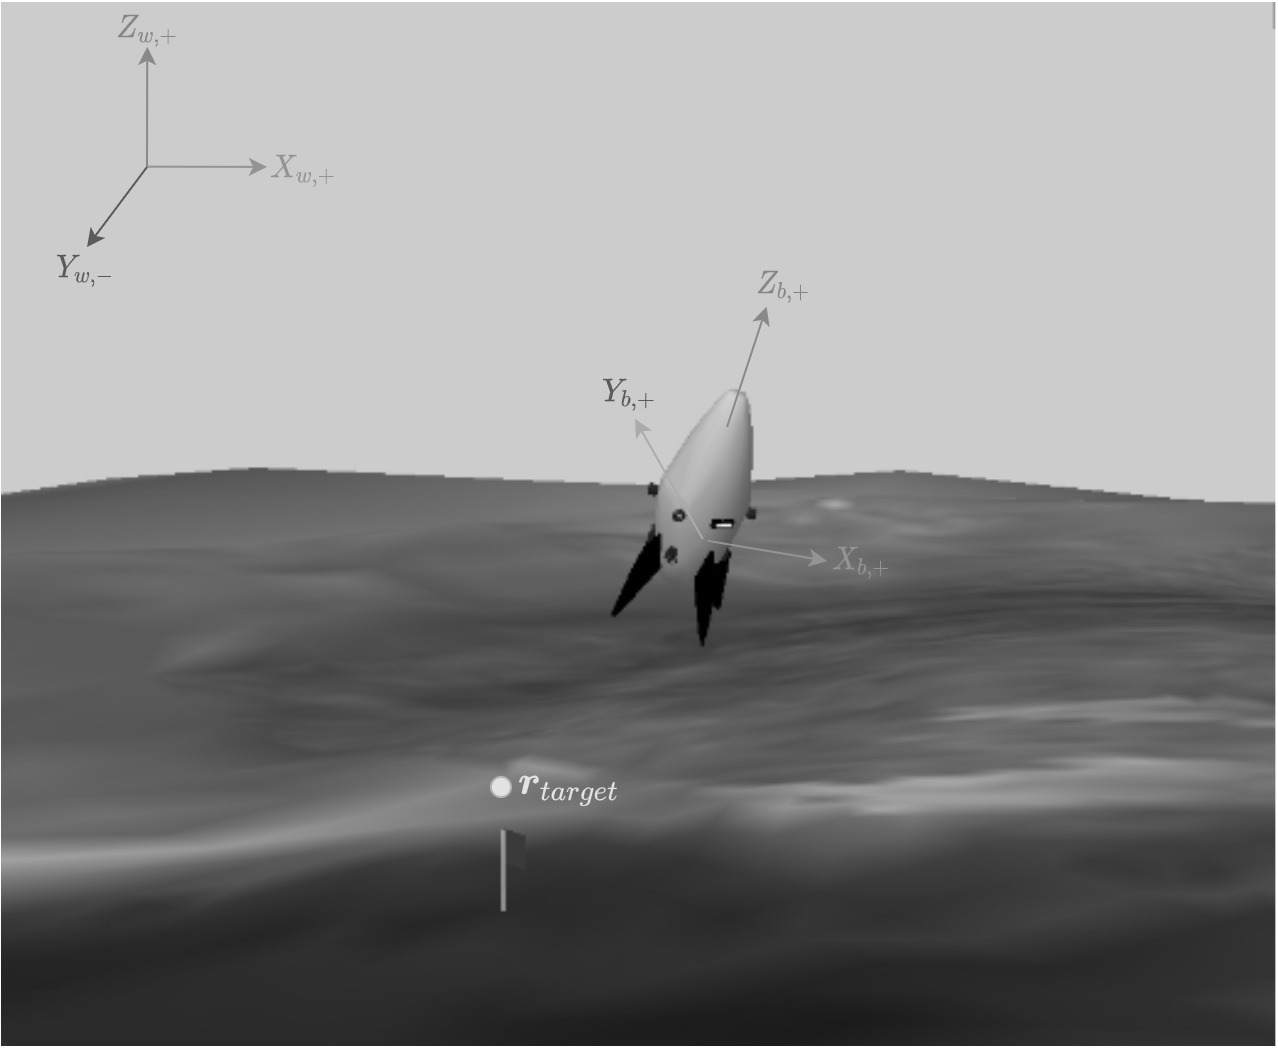
\includegraphics[width=.9\textwidth, keepaspectratio]{plant_geometry_1}
    \vspace*{2mm}
    \caption{illustration of \textit{body frame}, \textit{world frame}, and $r_{target}$}
    \label{fig:plant_geometry_1}
\end{figure}

Given a vehicle (a.k.a. the \textit{plant}) initially at a position $\boldsymbol{r}_{0}$ and oriented with the \textit{body frame} coordinates $(X_{b}, Y_{b}, Z_{b})$ all aligned with world frame coordinates $(X_{w}, Y_{w}, Z_{w})$ in free fall state, we'd try to land it to the target position $\boldsymbol{r}_{target}$ while minimizing propellant consumption during the flight, by maneuvering its thrusters. A successful landing is implied by \textit{all 4 legs touching ground and vehicle speed is damped down to $|\dot{\boldsymbol{r}}| < 10^{-2}$ m/s}. An illustration of the coordinates when the vehicle is near $r_{target}$ is presented by \cref{fig:plant_geometry_1}. 

Specifications of the \textit{plant} are introduced below. All variables in this article are assumed \textit{time varying} if not otherwise declared to be constant.

\begin{figure}[!htb]
    \centering
    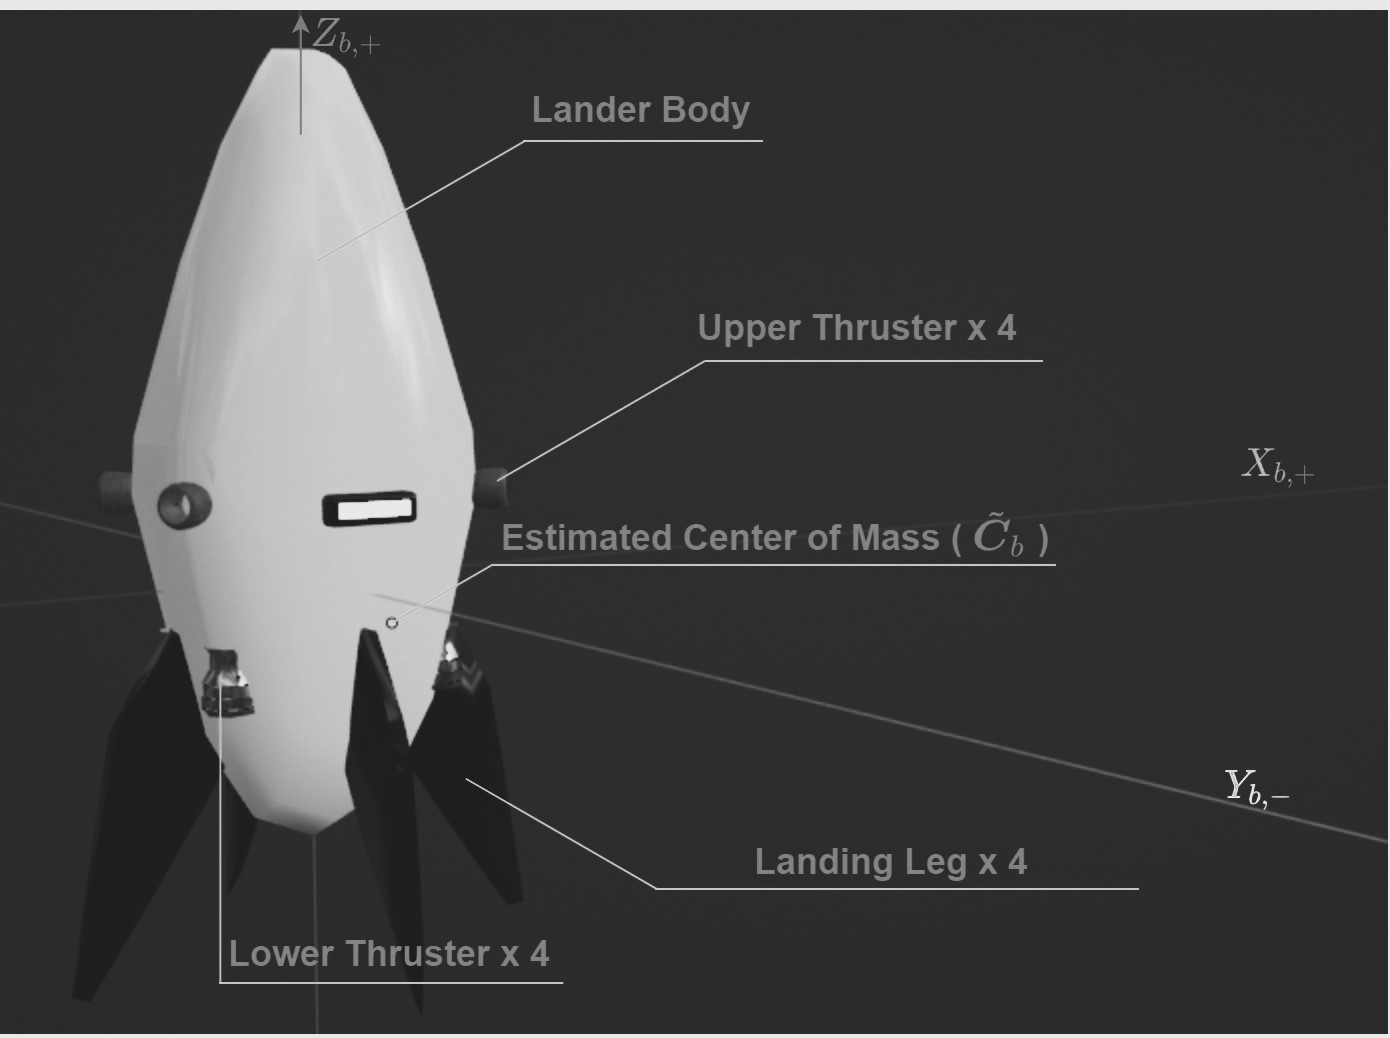
\includegraphics[width=.9\textwidth, keepaspectratio]{plant_geometry_2}
    \vspace*{2mm}
    \caption{vehicle specs part 1}
    \label{fig:plant_geometry_2}
\end{figure}

\begin{figure}[!htb]
    \centering
    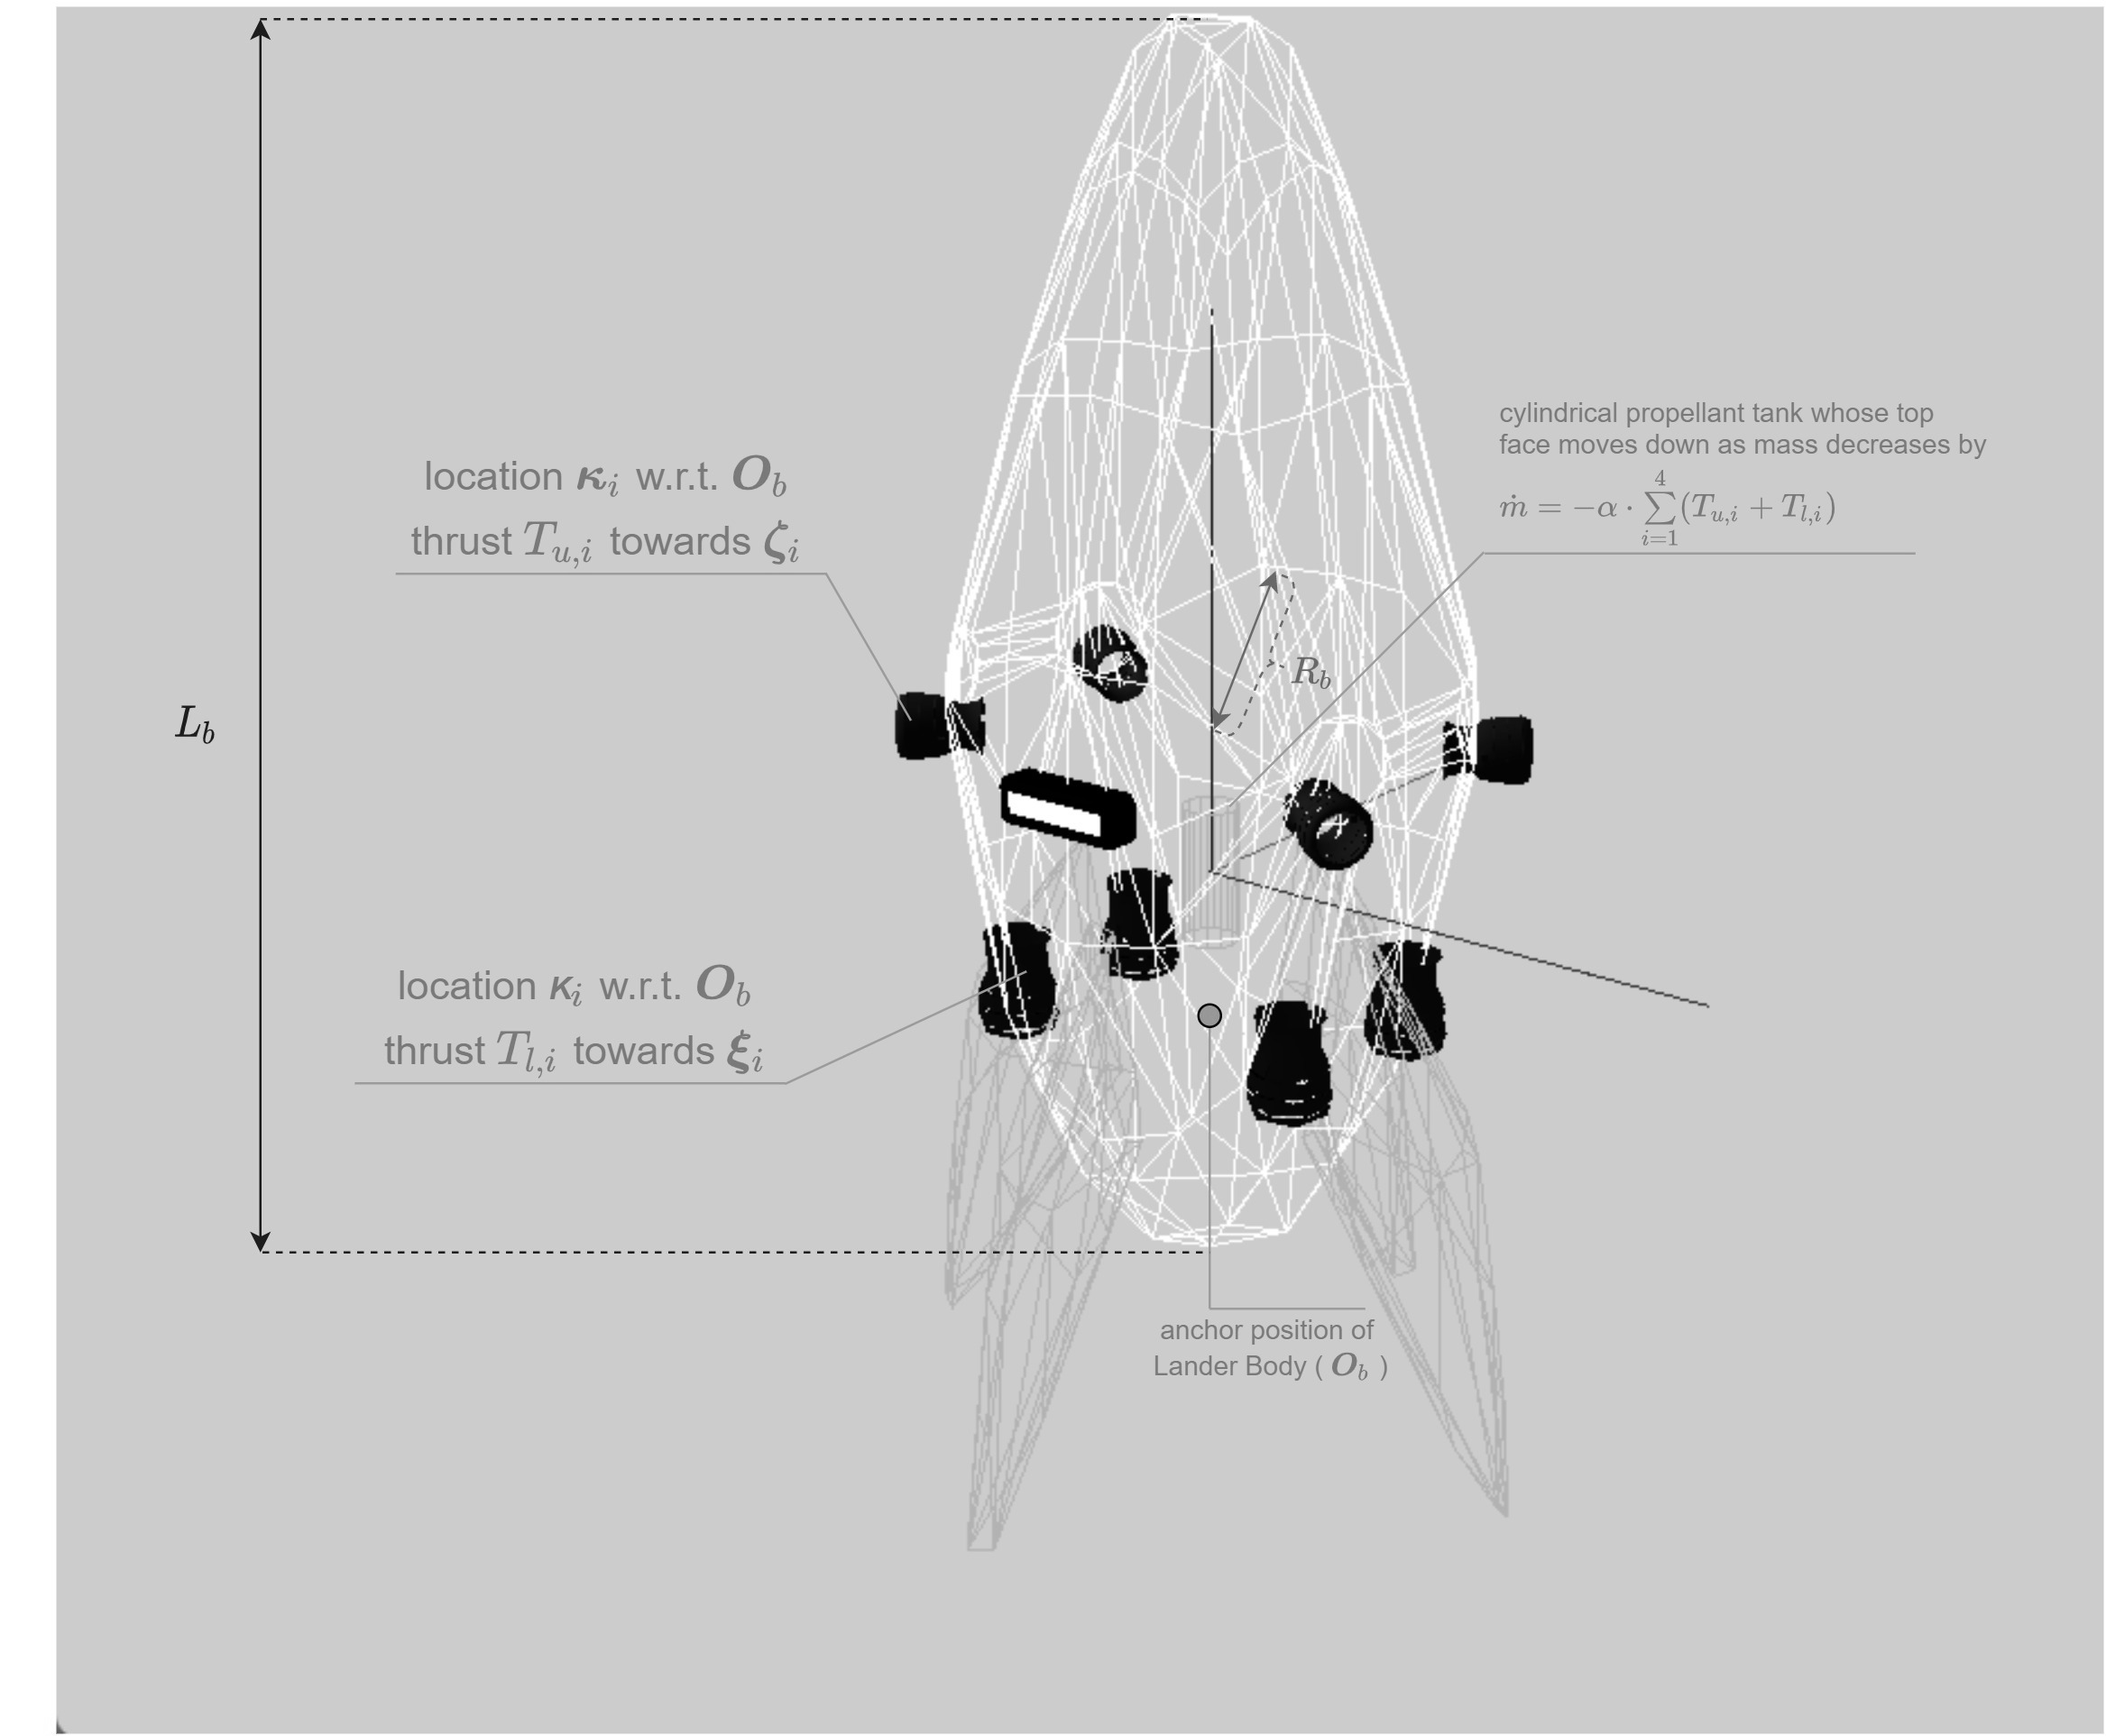
\includegraphics[width=.9\textwidth, keepaspectratio]{plant_geometry_3}
    \vspace*{2mm}
    \caption{vehicle specs part 2}
    \label{fig:plant_geometry_3}
\end{figure}

\begin{itemize} \label{eqs:hardwareconstraints}
    \item 1 ovoid shape \textit{Lander Body} with constant anchor position $\boldsymbol{O}_b$ (the geometric center of mesh), dry mass $m_b$ and dry inertia tensor $\boldsymbol{I}_{b, 0}$ in \textit{body frame}(i.e. always a diagonal matrix), major axis length $L_b$ and largest cross-section radius $R_b$ 
    \item 4 massless \textit{Upper Thrusters}, each located at $\boldsymbol{ \kappa }_{i}$ w.r.t. $\boldsymbol{O}_b$, thrusting towards $\boldsymbol{\zeta}_{i}$ in \textit{body frame} and with magnitude $T_{u,i} \in [\rho_1, \rho_2] \; \& \; \rho_1, \rho_2 > 0$ or being off, i.e. $T_{u,i} = 0$, 
    \item 4 massless \textit{Lower Thrusters}, each located at $\boldsymbol{ \upkappa } _{i}$ w.r.t. $\boldsymbol{O}_b$, thrusting towards $\boldsymbol{ \xi }_{i}$ in \textit{body frame} and with magnitude $T_{l,i} \in [\rho_1, \rho_2] \; \& \; \rho_1, \rho_2 > 0$ or being off, i.e. $T_{l,i} = 0$, 
    \item 1 cylindrical propellant tank (simplified to include fuel and oxidizer) inside the body that initially contributes to some of the total mass, when flying the propellant is consumed by a rate proportional to the thrusts, i.e. $\dot{m} = -\alpha \cdot \sum\limits_{i=1}^{4}{(T_{u,i} + T_{l,i})}$ where $m$ is the total mass of the whole lander; the decrement of $m$ changes the overall \textit{center of mass} during flight as well; the initial propellant mass is a constant $m_{prop,0}$
    \item 4 massless legs attached to the \textit{Lander Body} with revolute joints to provide support when landed, each leg is also shaped with a considerable air contacting area to favor disturbance from \cref{sec:windsim}    
    \item the rate of change in thrust magnitude of each thruster is unlimited
\end{itemize}

The navigation feedbacks of the \textit{plant} in \textit{world frame} are listed below.
\begin{enumerate}[label=\textbf{a.\arabic*}, itemsep=2pt] % or "nosep" in the place of "itemsep=..." to make even less vspace
  \item \label{eqs:r} $\begin{pmatrix} \boldsymbol{r} \\ \dot{\boldsymbol{r}} \end{pmatrix}$, position and velocity of the lander 
  \item \label{eqs:quat} $\begin{pmatrix} \boldsymbol{q} \\ \dot{\boldsymbol{q}} \end{pmatrix}$, attitude of the lander is represented by a quaternion $\boldsymbol{q}$ transforms $Z_{w,+}$ to align with the instantaneous $Z_{b,+}$ in \cref{fig:plant_geometry_1}, while $\dot{\boldsymbol{q}}$ is derived from the measured world frame angular velocity $\boldsymbol{\omega} = (\omega_x, \omega_y, \omega_z)$ by       
\[
    \boldsymbol{\dot{q}} = \frac{\boldsymbol{W} \cdot \boldsymbol{q}}{2}
\]

where 

$\boldsymbol{W} = 0 + \omega_x \cdot \boldsymbol{i} + \omega_y \cdot \boldsymbol{j} + \omega_z \cdot \boldsymbol{k}$; $\omega_x$ is the angular speed around $X_{w,+}$ in world frame (see \cref{fig:plant_geometry_1}), and similar arguments apply to $\omega_y$, $\omega_z$

  \item \label{eqs:m} $m$, total mass of the whole lander
\end{enumerate}

The state-space measurement $\boldsymbol{s}$ and maneuver $\boldsymbol{\Xi}$ of this \textit{plant} are denoted as follows.

\begin{equation} \label{eqs:state}
    \boldsymbol{s} \, := \begin{pmatrix} \boldsymbol{r} \\ \dot{\boldsymbol{r}} \\ \boldsymbol{q} \\ \boldsymbol{\dot{q}} \\ m \end{pmatrix}  
\end{equation}
\begin{equation} \label{eqs:maneuver}
    \boldsymbol{\Xi} \, := \begin{pmatrix} \boldsymbol{T}_{u} \\ \boldsymbol{T}_{l} \end{pmatrix}  
\end{equation}

\section{Controller Estimations}

\begin{figure*}[ht]
    \centering
    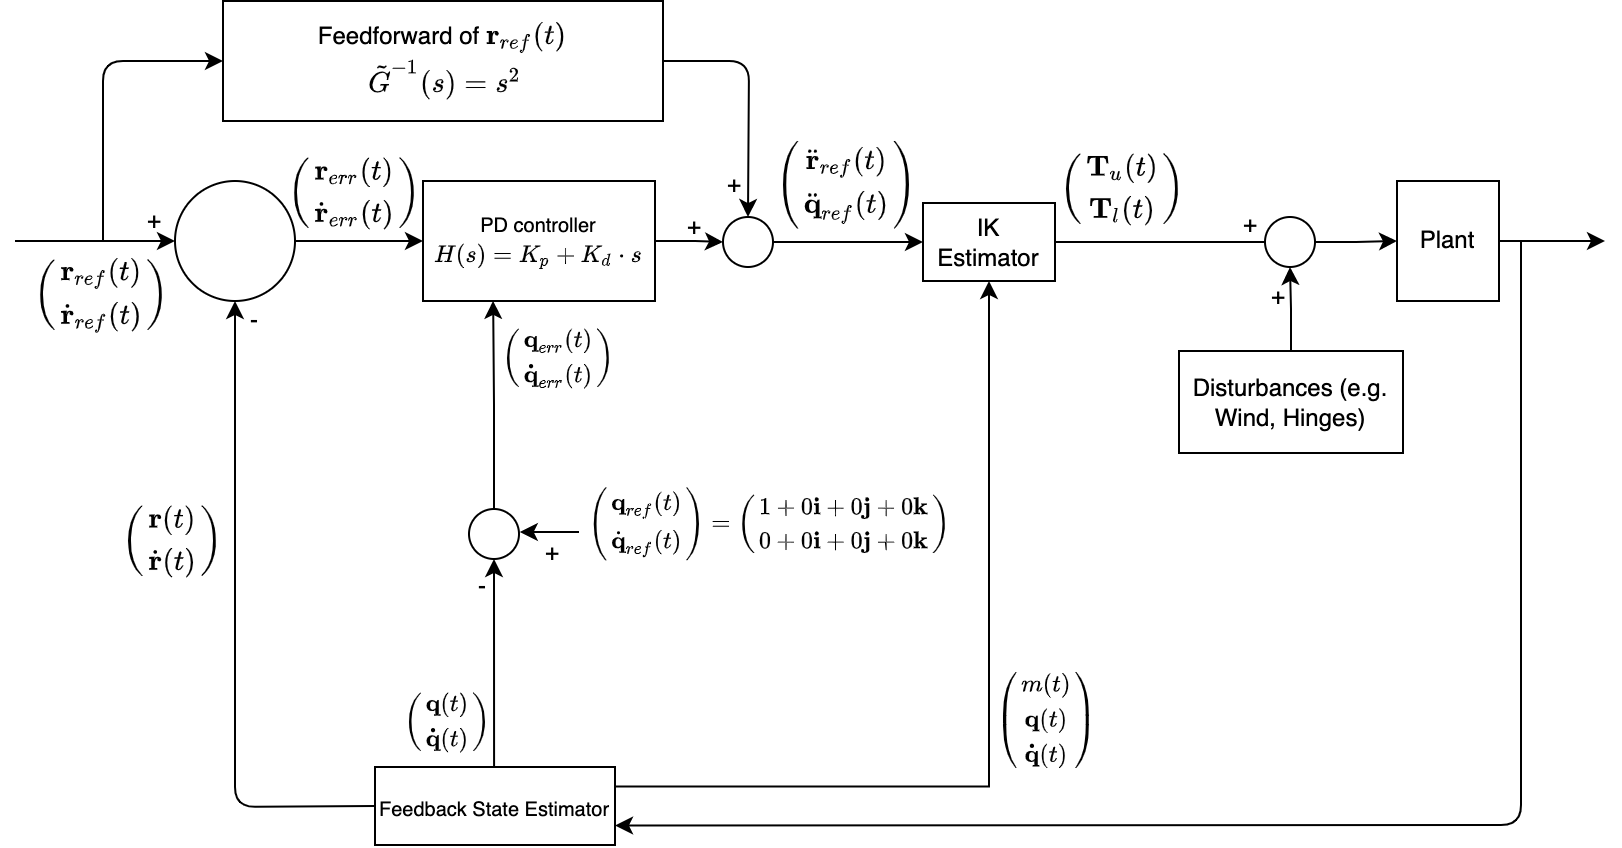
\includegraphics[width=.95\textwidth]{PD_feedforward_block}
    \vspace{5mm} 
    \caption{Block diagram of controller}
    \label{fig:PD_feedforward_block}
\end{figure*}

In \cref{fig:PD_feedforward_block} the \textit{IK Estimator} will take the following estimations to simplify the model.
\begin{enumerate}[label=\textbf{b.\arabic*}, itemsep=2pt]
    \item \label{eqs:bodyFrameCOM} $\tilde{\boldsymbol{C}}_b$, estimated \textit{center of mass} of the whole lander, which is a constant position in \textit{body frame}
    \item \label{eqs:bodyFrameInertia} $\tilde{\boldsymbol{I}}_b = \frac{m}{m_b} \cdot \boldsymbol{I}_{b, 0}$, estimated inertia tensor of the whole lander w.r.t. $\tilde{\boldsymbol{C}}_b$ in \textit{body frame} 
\end{enumerate}

The $\, \tilde{ } \,$ on \eqref{eqs:bodyFrameCOM} and \eqref{eqs:bodyFrameInertia} means that it's an estimation by the controller.

Therefore the controller estimated dynamics in \textit{body frame} would be

\footnotesize
\begin{equation} \label{eqs:accLinear}
\sum\limits_{i=1}^{4}{(T_{u,i} \cdot \boldsymbol{\zeta}_{i} + T_{l,i} \cdot \boldsymbol{\xi}_{i})} = \tilde{\boldsymbol{F}}_b     
\end{equation}

\begin{equation} \label{eqs:accIznewton}
\sum\limits_{i=1}^{4}{(\boldsymbol{\kappa}_{i} \times (T_{u,i} \cdot \boldsymbol{\zeta}_{i}) + \boldsymbol{\upkappa}_{i} \times (T_{l,i} \cdot \boldsymbol{\xi}_{i}))} = \tilde{\boldsymbol{M}}_b    
\end{equation}

where 

\begin{equation} \label{eqs:bodyFrameThrusts}
\tilde{\boldsymbol{F}}_b := \boldsymbol{q}^{-1} ((\ddot{\boldsymbol{r}} - \boldsymbol{g}) \cdot m) \boldsymbol{q}    
\end{equation}

\begin{equation} \label{eqs:bodyFrameTorque}
\tilde{\boldsymbol{M}}_b := \tilde{\boldsymbol{I}}_b \cdot \tilde{\boldsymbol{\beta}}_b - \tilde{\boldsymbol{\omega}}_b \times (\tilde{\boldsymbol{I}}_b \cdot \tilde{\boldsymbol{\omega}}_b)   
\end{equation}

\begin{equation} \label{eqs:accQuatBetaDef}
\tilde{\boldsymbol{\beta}}_b := \boldsymbol{q}^{-1} \cdot \dot{\boldsymbol{\omega}} \cdot \boldsymbol{q}
\end{equation}

\begin{equation} \label{eqs:accQuatOmegaDef}
\tilde{\boldsymbol{\omega}}_b := \boldsymbol{q}^{-1} \cdot \boldsymbol{\omega} \cdot \boldsymbol{q}
\end{equation}
\normalsize % recover normal font size

Wind dynamics will only be taken as \textit{disturbance}(\cref{sec:windsim}) as we don't have controllable fins in this problem.

\section{Guidance and Control} \label{sec:gdc}
\subsection{Guidance planning} \label{sec:gdp}

To land a vehicle from $\boldsymbol{r}_0$ to $\boldsymbol{r}_{target}$ with the hardware constraints given by \cref{eqs:hardwareconstraints}, we'd first employ a guidance algorithm to find a planned path $(\boldsymbol{r}_{ref}, \dot{\boldsymbol{r}}_{ref})$ for the vehicle to follow, while trying to minimize the total propellant consumption. 

The guidance algorithm here concerns only the trajectory of \textit{center of mass}, denote that

\begin{equation} \label{eqs:worldFrameThrusts}
\tilde{\boldsymbol{F}} = \boldsymbol{q} \cdot \tilde{\boldsymbol{F}}_b \cdot \boldsymbol{q}^{-1} 
\end{equation}

, we can rephrase the problem with fuel optimal goal to the following. Kindly note that \eqref{eqs:worldFrameThrusts} is indeed a reverse of \eqref{eqs:bodyFrameThrusts}. 

\textbf{Problem 1 (non-convex)} \label{prob:p1}

$\underset{t_f, \tilde{\boldsymbol{F}}}{\max} \; \tilde{m}(t_f) = \underset{t_f, \tilde{\boldsymbol{F}}}{\min} \int_{0}^{t_f} \|\tilde{\boldsymbol{F}}\| \cdot dt$

where
\[
\tilde{m}(0) = m_b + m_{prop,0}
\]
\[
\dot{\tilde{m}} = -\alpha \cdot \|\tilde{\boldsymbol{F}}\|
\]
\[
\tilde{\rho}_1 \le \|\tilde{\boldsymbol{F}}\| \le \tilde{\rho}_2 
\]
\[
\dot{\boldsymbol{r}}(t_f) = \dot{\boldsymbol{r}}(0) = \boldsymbol{0}
\]
\[
\boldsymbol{r}(0) = \boldsymbol{r}_0
\]
\[
\boldsymbol{r}(t_f) = \boldsymbol{r}_{target}
\]
\[
\ddot{\boldsymbol{r}} = \frac{\tilde{\boldsymbol{F}}}{\tilde{m}} + \boldsymbol{g}
\]
\[
\tilde{m}(t_f) \ge m_b + (1 - \lambda) \cdot m_{prop,0}
\]
\[
r_z \ge r_{target,z} 
\]

Kindly note there's an empirically chosen constant $\lambda$, and an estimation $\tilde{m}$ instead of $m$ is used here because in general $\dot{\tilde{m}} \le \dot{m}$, thus we can be more conservative to constrain that $\lambda \le 0.7$, i.e. plan to use only up to $70\%$ of the propellant. 

The new thrust bounds $\tilde{\rho}_1$, $\tilde{\rho}_2$ could've been estimated from $\rho_1$, $\rho_2$, $\rho_{side,1}$, $\rho_{side,2}$, $\Phi_{min}$, $\Phi_{max}$ analytically, but in practice it's fair to just take the following approximations because we expect the main engine to contribute most to the thrust magnitude.
\[
\tilde{\rho}_1 = \rho_1, \; \tilde{\rho}_2 = \rho_2
\]


According to \cite{cvxpow, losslesscvx} \textit{Problem 1} is non-convex but can be losslessly convexified to the following \textit{Second Order Cone Programming (SOCP)}\cite{alizadeh2003second}.

\textbf{Problem 2 (SOCP)} \label{prob:p2}

$\underset{t_f, \boldsymbol{u}, \sigma}{\min} \; \int_{0}^{t_f} \sigma \cdot dt$

where 
\small
\begin{equation}
\eta(0) = \ln(m_b + m_{prop,0})
\end{equation}
\begin{equation}
\dot{\boldsymbol{r}}(t_f) = \dot{\boldsymbol{r}}(0) = \boldsymbol{0}
\end{equation}
\begin{equation}
\boldsymbol{r}(0) = \boldsymbol{r}_0
\end{equation}
\begin{equation}
\boldsymbol{r}(t_f) = \boldsymbol{r}_{target}
\end{equation}
\begin{equation}
\ddot{\boldsymbol{r}} = \boldsymbol{u} + \boldsymbol{g}
\end{equation}
\begin{equation} 
\mu_1 (1-(\eta-\eta_0)+\frac{(\eta-\eta_0)^2}{2}) \le \sigma \le \mu_2 (1-(\eta-\eta_0)) 
\end{equation}
\begin{equation}
\eta_0 \le \eta \le \ln(m_b + m_{prop,0} - \alpha \cdot \tilde{\rho}_1 \cdot t)
\end{equation}
\begin{equation} \|\boldsymbol{u}\| \le \sigma \end{equation}
\begin{equation} \dot{\eta} = -\alpha \cdot \sigma \end{equation}
\begin{equation}
\eta(t_f) \ge \ln(m_b + (1 - \lambda) \cdot m_{prop,0})
\end{equation}
\begin{equation} 
r_z \ge r_{target,z}
\end{equation}
\normalsize

by introducing new variables
\[
\boldsymbol{u} \, := \frac{\tilde{\boldsymbol{F}}}{\tilde{m}}
\]
\[
\eta \, := \ln(\tilde{m})
\]
\[
\eta_0 \, := \ln(m_b + m_{prop,0} - \alpha \cdot \tilde{\rho}_2 \cdot t)
\]
\[
\mu_1 \, := \tilde{\rho}_1 \cdot e^{-\eta_0}, \mu_2 = \tilde{\rho}_2 \cdot e^{-\eta_0}
\]

The following \textit{low speed} constraints can be added to \textit{Problem 2} without breaking the SOCP compliance.  
\begin{equation} 
\dot{\boldsymbol{r}}_z \le given \, descending \, speed \, limit
\end{equation}
\begin{equation} 
|\ddot{\boldsymbol{r}}_z| \le given \, descending \, acceleration \, limit
\end{equation}

When given a certain termination time-of-flight $t_f$ and discretized about $t$, \textit{Problem 2} can be numerically solved in an efficient manner by using SOCP specific solvers like \textit{Embedded Conic Solver (ECOS)}\cite{domahidi2013ecos} in search for a feasible $t_f$ will be in range $t_f \in [\frac{m_b \cdot |\dot{\boldsymbol{r}}(0)|}{\rho_2}, \frac{m_{prop,0}}{\rho_1}]$.

\subsection{Controller design} \label{sec:controllerdesign}

Given the guidance path $\begin{pmatrix} \boldsymbol{r}_{ref} \\ \dot{\boldsymbol{r}}_{ref} \end{pmatrix}$, the vehicle needs a control algorithm to actually follow the path for landing. The control algorithm aims to find proper thrusts $\boldsymbol{T}_{u}, \boldsymbol{T}_{l}$ whenever the controller is active, and these thrusts are employed by the thrusters to apply dynamics to the vehicle.     

The \eqref{eqs:accLinear}, \eqref{eqs:accIznewton} w.r.t. \eqref{eqs:state} \& \eqref{eqs:maneuver} form a \textit{Multi Input Multi Output (MIMO)} system, an intuitive choice would be to obtain a linearized $\boldsymbol{\dot{q}} = \boldsymbol{A} \cdot \boldsymbol{q} + \boldsymbol{B} \cdot \boldsymbol{w}$ from \eqref{eqs:accLinear}, \eqref{eqs:accIznewton} at a chosen trim point, then apply a Model Predictive Control by scoring proximity to $\begin{pmatrix} \boldsymbol{r}_{ref} \\ \dot{\boldsymbol{r}}_{ref} \end{pmatrix}$. 

However there's inconvenience for linearizing this model. Only part of $\boldsymbol{q}$ can be linearized because $\dot{m} \ne 0$ during flight, and a non-hover flight might remove $\begin{pmatrix} \boldsymbol{r} \\ \dot{\boldsymbol{r}} \end{pmatrix}$ from linearizable parts over all time\cite{kim2020modeling}, resulting in extra complications in design of the whole controller as the non-linearized parts are not decoupled.     

For this problem the relatively simple PID controllers with the non-linear model suffices to work to satisfaction. By decoupling inputs and outputs into several \textit{Single-Input-Single-Output (SISO)} PID controllers, we avoid empirically guessing any cross coupled factors for \eqref{eqs:maneuver} w.r.t. \eqref{eqs:r}, \eqref{eqs:quat}, \eqref{eqs:m}, as shown in the figure below.

\begin{figure*}[ht] 
    \centering
    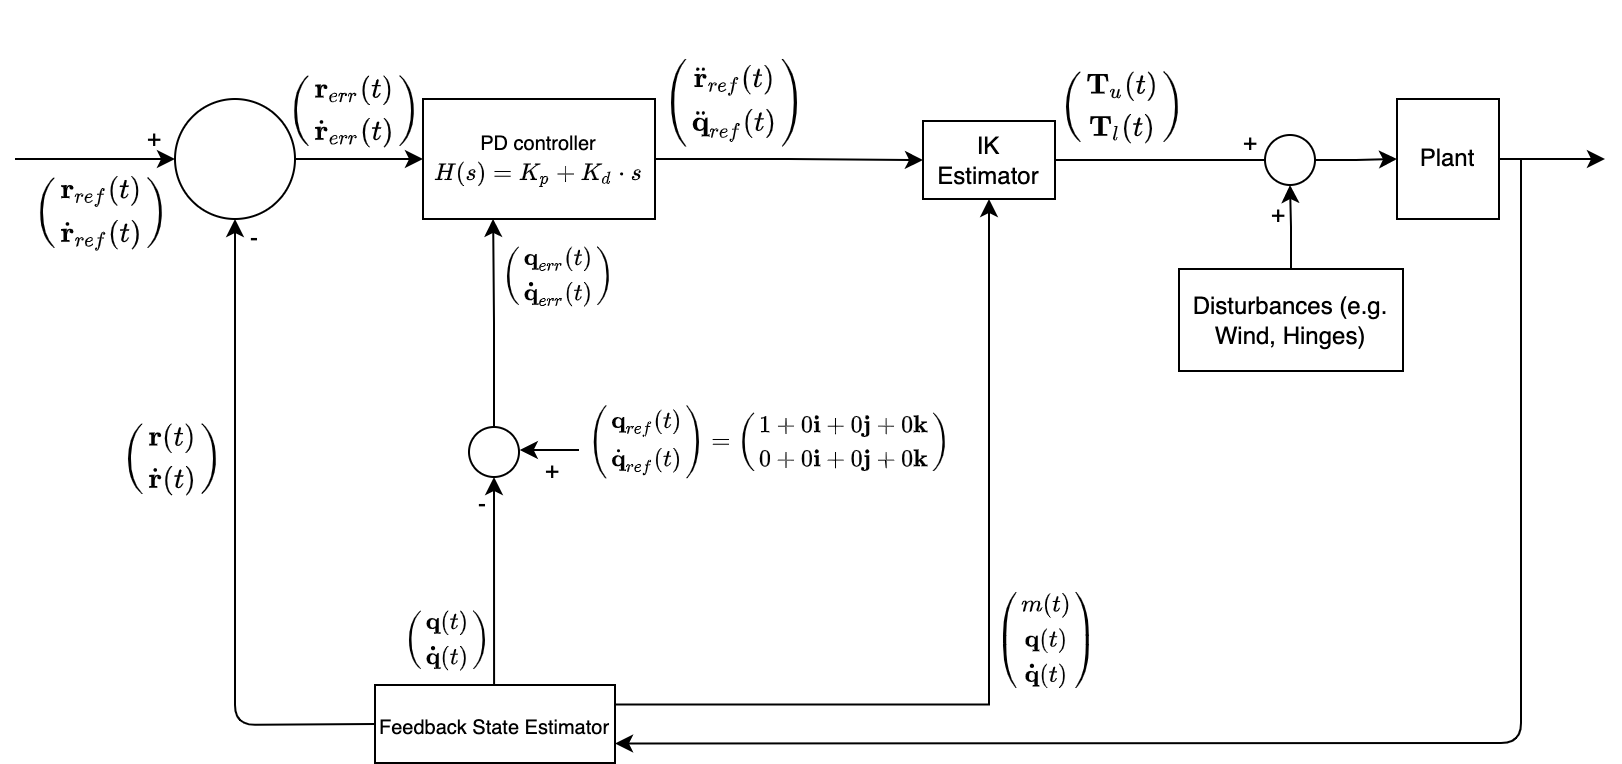
\includegraphics[width=.95\textwidth]{PD_block}
    \vspace*{2mm}
    \fnote{* in \cref{fig:PD_feedforward_block} a feedforward route $\tilde{G}^{-1}(s) = s^2$ which reduces delay in $\dot{\boldsymbol{r}}$ tracking $\dot{\boldsymbol{r}}_{ref}$\cite{visioli2004new} is added}
    \vspace*{5mm}
    \caption{Block diagram of non-feedforward controller}
    \label{fig:PD_block}
\end{figure*}

First, each of the SISO PID controllers would seek the proper $\boldsymbol{r}_{ref}(t_{ref})$ as the instantaneous reference location to track by KD-tree search\cite{maneewongvatana1999analysis}, and is just a classical PD controller responsible for position or attitude control 
\begin{equation} \label{eqs:Gtilde}
\tilde{G}(s) = \frac{1}{s^2}
\end{equation}
\begin{equation} \label{eqs:Hr}
H_{\boldsymbol{r}}(s) = K_{p,\boldsymbol{r}} + s \cdot K_{d,\boldsymbol{r}} 
\end{equation}
\begin{equation} \label{eqs:Hquat}
H_{\boldsymbol{q}}(s) = K_{p,\boldsymbol{q}} + s \cdot K_{d,\boldsymbol{q}}
\end{equation}
\begin{equation} \label{eqs:closedlooptf1}
\mathcal{L}\{ \boldsymbol{r} \}= \frac{\tilde{G} \cdot H_{\boldsymbol{r}}}{1 + \tilde{G} \cdot H_{\boldsymbol{r}}} \cdot \mathcal{L}\{ \boldsymbol{r}_{ref} \}
\end{equation}
\begin{equation} \label{eqs:closedlooptf2}
\mathcal{L}\{ \boldsymbol{q} \}= \frac{\tilde{G} \cdot H_{\boldsymbol{q}}}{1 + \tilde{G} \cdot H_{\boldsymbol{q}}} \cdot \mathcal{L}\{ \boldsymbol{q}_{ref} \}
\end{equation}

where $\mathcal{L}\{\cdot\}$ indicates the Laplace transform. 

The $\, \tilde{ } \,$ on \eqref{eqs:Gtilde} means that it's an estimation of what the \textit{IK Estimator} and \textit{Plant} steps together would approximately achieve
\[
\begin{pmatrix} \boldsymbol{r}(t) \\ \boldsymbol{q}(t) \end{pmatrix} = \int_0^t \int_0^t \begin{pmatrix} \ddot{\boldsymbol{r}}_{ref}(\tau) \\ \ddot{\boldsymbol{q}}_{ref}(\tau) \end{pmatrix} \cdot d \tau^2
\]
in good fidelity. 

That \eqref{eqs:Gtilde} being a \textit{no delay, no damp double integrating} transfer function makes it a peculiar second order system to design the PID controller. In a wellknown case    
\begin{equation} \label{GtildeAlt}
  \tilde{G}_{alt}(s) = \frac{e^{-\gamma s}}{(\delta_1 s + 1)(\delta_2  s + 1)}
\end{equation}
, simple IMC approach to estimate $2^{nd}$-order approximator and then a single parameter tunable PID controller is proposed in \cite{skogestad2012simc}. However in a simulation environment without air dynamics, \eqref{eqs:Gtilde} will remain as-is and thus even the treatments in \cite{grimholt2016optimal, ruscio2017tuning} wouldn't be applicable due to $\gamma = 0$. 

Aiming at an analytical approach to determine the variables in \eqref{eqs:Hr}, \eqref{eqs:Hquat} and knowing that derivative action is necessary for stabilization for \eqref{eqs:Gtilde}\cite{grimholt2016optimal}, every PID controller is limited to be a PD controller in our approach and the steady state error will instead be complemented by a feedforward route. 

To compute proper $K_{p, \boldsymbol{r}}$ and $K_{d, \boldsymbol{r}}$, as we're also constrained by 
$T_{settle} < t_f$ from the \cref{sec:gdp}, an analytical $\tilde{T}_{settle}(K_p, K_d)$ for each dimension is preferable given requirements of the unit step response of \eqref{eqs:closedlooptf1} 
\begin{enumerate}[label=\textbf{c.\arabic*}, itemsep=2pt]
    \item \label{eqs:setrange} $\lambda_{settle}$, the settled response amplitude ratio threshold       
    \item \label{eqs:pOS} $pOS_{0}$, the expected peak overshoot
    \item \label{eqs:Tsettle} $\tilde{T}_{settle, 0} = (0.6 \cdot t_f)$, the intersection of amplitude envelope of $\mathcal{L}^{-1}\{\frac{\tilde{G} \cdot H_{\boldsymbol{r}}}{1 + \tilde{G} \cdot H_{\boldsymbol{r}}} \cdot \frac{1}{s}\}$ and the $SettlingTimeThreshold$ horizon
\end{enumerate}
, to numerically find a fit for both
\begin{enumerate}[label=\textbf{d.\arabic*}, itemsep=2pt]
    \item $|\frac{\tilde{T}_{settle}(K_{p,\boldsymbol{r}}, \, K_{d,\boldsymbol{r}})}{\tilde{T}_{settle, 0}} - 1| < 0.05$, and
    \item $|\frac{pOS(K_{p,\boldsymbol{r}}, \, K_{d,\boldsymbol{r}})}{pOS_{0}} - 1| < 0.05$
\end{enumerate}
, where the analytical form of $\tilde{T}_{settle}(\cdot, \cdot)$ and $pOS(\cdot, \cdot)$ can be calculated by symbolic calculation tools. 

Next, given $\begin{pmatrix} \ddot{\boldsymbol{r}}_{ref} \\ \ddot{\boldsymbol{q}}_{ref} \end{pmatrix}$ computed by the \textit{PD Controller} step, the \textit{IK Estimator} will compute computes the instantaneous \eqref{eqs:maneuver} numerically in \textit{body frame} for maneuver. Details will be described in \cref{sec:ikestimator}. 

Lastly, the \textit{Plant} in simulation will guarantee to clip $T_{l,i} \in [\rho_1, \rho_2]$ and $T_{u,i} \in [\rho_1, \rho_2]$ before stepping in the physics engine.

\subsection{IK Estimator} \label{sec:ikestimator}
Following the PID controller output, the proposed \textit{IK Estimator} computes    

\begin{equation} \label{eqs:qdotdotToBeta}
    \boldsymbol{\dot{\omega}} = 2 \cdot ( \boldsymbol{\ddot{q}} \cdot \boldsymbol{q} - (\boldsymbol{\dot{q}} \cdot \boldsymbol{q}^{-1})^2 )  
\end{equation}

, and then the desired instantaneous $\tilde{\boldsymbol{F}}_b$ and $\tilde{\boldsymbol{M}}_b$ by \eqref{eqs:bodyFrameThrusts}, \eqref{eqs:bodyFrameTorque}. 

Eventually \eqref{eqs:maneuver} is numerically solved to approximately fulfill \eqref{eqs:accLinear}, \eqref{eqs:accIznewton} as a minimization problem

\textbf{Problem 3 (thrust lower bound loosen)} \label{prob:p3}
\begin{equation}
\underset{\boldsymbol{T}'_{u}, \boldsymbol{T}'_{l}}{\min} \left| \begin{pmatrix} \sum\limits_{i=1}^{4}{(T'_{u,i} \cdot \boldsymbol{\zeta}_{i} + T'_{l,i} \cdot \boldsymbol{\xi}_{i})} - \tilde{\boldsymbol{F}}_b \\ \sum\limits_{i=1}^{4}{(\boldsymbol{\kappa}_{i} \times (T'_{u,i} \cdot \boldsymbol{\zeta}_{i}) + \boldsymbol{\upkappa}_{i} \times (T'_{l,i} \cdot \boldsymbol{\xi}_{i}))} - \tilde{\boldsymbol{M}}_b \end{pmatrix} \right|
\end{equation}

for constraints 

\begin{equation*}
T'_{u,i} \in [0, \rho_2]
\end{equation*}
\begin{equation*}
T'_{l,i} \in [0, \rho_2]
\end{equation*}

\begin{equation} 
\sum\limits_{i=1}^{4}{(T'_{u,i} \cdot \boldsymbol{\zeta}_{i} + T'_{l,i} \cdot \boldsymbol{\xi}_{i})} = \tilde{\boldsymbol{F}}_b     
\tag{\ref{eqs:accLinear} revisited} % comment out this line when using Pandoc for conversion 
\end{equation}

\begin{equation} 
\sum\limits_{i=1}^{4}{(\boldsymbol{\kappa}_{i} \times (T'_{u,i} \cdot \boldsymbol{\zeta}_{i}) + \boldsymbol{\upkappa}_{i} \times (T'_{l,i} \cdot \boldsymbol{\xi}_{i}))} = \tilde{\boldsymbol{M}}_b    
\tag{\ref{eqs:accIznewton} revisited} % comment out this line when using Pandoc for conversion
\end{equation}

The overdetermined linear system \eqref{eqs:accLinear}, \eqref{eqs:accIznewton} could be violated to a certain extent at some instant of time, thus \textit{Problem 3} is solved by \textit{Sequential Least Squares Programming (SLSQP)}\cite{kraft1994algorithm} which can allow violation of constraints to certain extent for engineering practice. 

For any solution $\boldsymbol{T}'_{u}, \boldsymbol{T}'_{l}$ to \textit{Problem 3}, each value $T'_{u,i}$, $T'_{l,i}$ will be clipped into $[\rho_1, \rho_2]$ or $0$ by the simulation thread to guarantee that thrust magnitude constraints are never violated. 

After clipping $\boldsymbol{T}'_{u}, \boldsymbol{T}'_{l}$ into $\boldsymbol{T}_{u}, \boldsymbol{T}_{l}$ ($T_{u,i} \in [\rho_1, \rho_2]$ or $T_{u,i} = 0$, $T_{l,i} \in [\rho_1, \rho_2]$ or $T_{l,i} = 0$), the violation is chosen to be recorded by 
\begin{equation} \label{eqs:ikcv}
|\boldsymbol{Q}| := \left| \begin{pmatrix} \sum\limits_{i=1}^{4}{(T_{u,i} \cdot \boldsymbol{\zeta}_{i} + T_{l,i} \cdot \boldsymbol{\xi}_{i})} - \tilde{\boldsymbol{F}}_b \\ (\sum\limits_{i=1}^{4}{(\boldsymbol{\kappa}_{i} \times (T_{u,i} \cdot \boldsymbol{\zeta}_{i}) + \boldsymbol{\upkappa}_{i} \times (T_{l,i} \cdot \boldsymbol{\xi}_{i}))} - \tilde{\boldsymbol{M}}_b)/\mathcal{J} \end{pmatrix} \right|
\end{equation}

where $\mathcal{J} \, (unit: \, m)$ is the normalizing factor that makes all dimensions of $\boldsymbol{Q}$ of same unit $N$. Discussion of $|\boldsymbol{Q}|$ will be presented in \cref{sec:results}.  

\section{Disturbances} \label{sec:disturbance}
\subsection{Scheduling uncertainty}
In runtime, a controller thread is scheduled independently from the physics simulation thread, where the physics simulation thread is responsible for applying the thrusts (determined by controller thread) as impulses during the discrete time step. Each thread gets uncertainty for the inter-tick duration as well as order of scheduling, thus resulting in different outputs for tests of same inputs.      

\begin{figure}[!ht]
    \centering
    \includegraphics[width=10.0cm, keepaspectratio]{Schedulings}
    \vspace*{3mm}
    \caption{Different possible schedulings of simulation thread and controller thread}
    \label{fig:schedulings}
\end{figure}
In \cref{sec:simtest} the tests are run on a \textit{non-Realtime Operating System}, where an unexpected order of scheduling could significantly degrade the performance of controlling. For example if the physics simulation thread ticks consecutively 3 times with an outdated set of thrusts without a new tick of controller thread to measure and update as shown in \textit{bad scheduling} of \cref{fig:schedulings}, the \textit{plant} might become difficult to land by following the guidance path. The controller thread could be scheduled such that it ticks at a specified minimum frequency, e.g. 120 fps, in a deterministic manner if the tests were run on a \textit{Realtime Operating System}.  

The following records are kept for scheduling uncertainty.
\begin{enumerate}[label=\textbf{e.\arabic*}, itemsep=2pt] % or "nosep" in the place of "itemsep=..." to make even less vspace
  \item \label{eqs:simCnt} $simCnt$, the accumulated count of physics simulation thread ticks  
  \item \label{eqs:ctrlCnt} $ctrlCnt$, the accumulated count of controller thread ticks
  \item \label{eqs:tickRatio} $\mathcal{T} := 1+sign(\frac{d(simCnt/ctrlCnt)}{dt})$, the time series for \textit{bad scheduling} occurrences    
\end{enumerate}

Discussion of $\mathcal{T}$ will be presented in \cref{sec:results}.

\subsection{Fluctuating \textit{center of mass} and \textit{inertia}}
As shown in \cref{fig:plant_geometry_3} of \cref{sec:problem}, the top face of the cylindrical propellant tank will be lowered as the propellant mass decreases, resulting in a time varying \textit{center of mass} $\boldsymbol{C}_b$ and \textit{inertia} $\boldsymbol{I}_b$ in \textit{body frame}. 

The fluctuating \textit{center of mass} and \textit{inertia} are accounted as \cref{eqs:bodyFrameCOM,eqs:bodyFrameInertia} respectively by the controller.

\subsection{Simulated wind} \label{sec:windsim}
The simulated wind is simplified as inviscid, incompressible and irrotational everywhere, imposing forces on the triangular mesh surface of the lander. 

\begin{figure}[!ht]
    \centering
    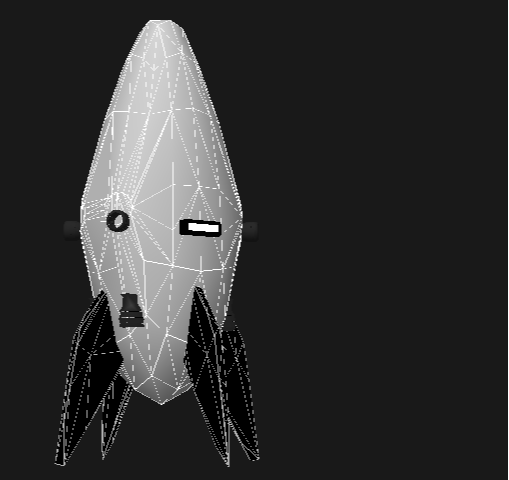
\includegraphics[width=10.0cm, keepaspectratio]{WindSimMesh}
    \vspace*{3mm}
    \caption{Triangular mesh surface of the lander}
    \label{fig:WindSimMesh}
\end{figure}

On each triangle surface with area $S_i$ and norm $\boldsymbol{n}_i$, the forces imposed by the wind in \textit{world frame} are

\footnotesize
\[
\boldsymbol{f}_{drag} = - 0.6 \cdot \rho_{air} \cdot \boldsymbol{v}_{d} \cdot (\boldsymbol{S}_i \cdot \boldsymbol{v}_{d})   
\]
\[
\boldsymbol{f}_{lift} = \begin{cases}
                              0.4 \cdot \rho_{air} \cdot (\boldsymbol{S}_i \times \boldsymbol{v}_{d} \times \boldsymbol{n}_{d}), & \text{if}\ 0 < \boldsymbol{n}_{d} \cdot \boldsymbol{n}_i < 0.98 \\
                              \boldsymbol{0}, & \text{otherwise}
                        \end{cases}
\]
\normalsize

where 
\[
\boldsymbol{S}_i = S_i \boldsymbol{n}_i   
\]
\[
\boldsymbol{v}_{d} = \boldsymbol{\dot{r}} - \boldsymbol{v}_{wind}    
\]
\[
\boldsymbol{n}_{d} = \frac{\boldsymbol{v}_{d}}{|\boldsymbol{v}_{d}|}    
\]

The simulated wind is not accounted by the controller either.

\section{Simulation Test} \label{sec:simtest}
Simulation tests were conducted for 6 \textit{input sets}, each \textit{input set} has a unique combination of (\textit{wind profile \#}, $r_{0}$, $r_{target}$). 

All \textit{input sets} share the same configuration of constants in \cref{sec:const}. Each \textit{input set} contains 20 \textit{episodes} and all episodes under the same \textit{input set} share the same (\textit{wind profile \#}, $r_{0}$, $r_{target}$) and thus the same computed guidance path $\begin{pmatrix} \boldsymbol{r}_{ref} \\ \dot{\boldsymbol{r}}_{ref} \end{pmatrix}$. 

For each \textit{input set}, 4 major performance indicators $\overline{\Delta}(\boldsymbol{r})$, $\overline{\Delta}(\boldsymbol{\dot{r}})$, $\overline{\Delta}(|\boldsymbol{q}|)$, $\overline{\Delta}(m)$ will be presented. Moreover, we examined several possible causes for the relatively poor alignment of $m \; v.s. \; m_{ref}$ by discussing $Pr(\mathcal{T}, \frac{\dot{m}}{\dot{m}_{ref}})$ and ${Pr}(|\boldsymbol{Q}|, \frac{\dot{m}}{\dot{m}_{ref}})$.  

Here $\Delta$ denotes \textit{Root Mean Square Error (RMSE)} for the measured values is w.r.t. corresponding guidance value, and $Pr$ denotes \textit{Pearson's correlation coefficient}\cite{student1908probable}, and the $\text{ } \, \bar{} \, \text{ }$ of each column in \textit{Outputs} indicates that it's averaged from 20 episodes of the same inputs over $[0, \text{measured} \; t_{f}] \; seconds$. 

\subsection{Constants} \label{sec:const}

All using SI units, while dimensions and weights are referencing the Masten XL-1 profile.
\footnotesize
\begin{enumerate}[label=\textbf{f.\arabic*}, itemsep=2pt]
    \item $\boldsymbol{g} = \begin{pmatrix} 0 \\ 0 \\ -9.81 \end{pmatrix} \, m^2/s, \, \text{same gravity as the earth}$    
    \item $L_b = 4.424 \, m, \, R_b = 0.8755 \, m, \mathcal{J} = 1.0 \, m$
    \item $m_b = 728.28 \, kg, \, m_{prop,0} = 1699.32 \, kg$
    \item $\rho_1 = 7282.8 \, N, \, \rho_2 = 24276.0 \, N$
    \item $\boldsymbol{\kappa} = \begin{pmatrix} 0.86602 & -0.86602 & -0.86602 & 0.86602 \\ 0.5 & 0.5 & -0.5 & -0.5 \\ 0.5 & 0.5 & 0.5 & 0.5 \end{pmatrix} m$
    \item $\boldsymbol{\upkappa} = \begin{pmatrix} 0.60622 & -0.60622 & -0.60622 & 0.60622 \\ 0.35 & 0.35 & -0.35 & -0.35 \\ -0.5 & -0.5 & -0.5 & -0.5 \end{pmatrix} m$
    \item \begingroup % increase matrix vertical spacing
            \renewcommand*{\arraystretch}{1.5}
            $\boldsymbol{\zeta} = \begin{pmatrix} cos\frac{\pi}{5} & cos\frac{4\pi}{5} & cos\frac{6\pi}{5} & cos\frac{9\pi}{5} \\ sin\frac{\pi}{5} & sin\frac{4\pi}{5} & sin\frac{6\pi}{5} & sin\frac{9\pi}{5} \\ 0 & 0 & 0 & 0 \end{pmatrix}$
          \endgroup 
    \item $\boldsymbol{\xi} = \begin{pmatrix} 0 & 0 & 0 & 0 \\ 0 & 0 & 0 & 0 \\ 1 & 1 & 1 & 1 \end{pmatrix}$
    \item $\lambda_{settle} = 0.05, \, pOS_{0} = 0.08, \, \tilde{T}_{settle, 0} = 1.77 \, s$, according to \cref{sec:controllerdesign} the controller parameters are $K_{p,\boldsymbol{r}} = K_{p,\boldsymbol{q}} = 3.00, \, K_{d,\boldsymbol{r}} = K_{d,\boldsymbol{q}} = 5.00$
    \item $\text{guidance discretization fps} =  15 \, \text{frames/s}$
    \item $\text{simulation \& renderer fps} =  60 \, \text{frames/s}$
\end{enumerate}
\normalsize

\begin{table}[htb]
\centering
\caption{Wind profiles}
\label{tab:windprofiles}
\vspace{2mm}
\begin{tabular}{c c c}
    \hline
    \text{wind\#} & $\boldsymbol{v}_{wind}(\boldsymbol{r}, t) \; m/s$ & $\rho_{air}(\boldsymbol{r}, t) \; kg/m^3$ \\
    \hline
    \tiny
    & & \\ % an empty row for some top padding
    $\#1$ & \text{const.} $\begin{pmatrix} 0.0 \\ 0 \\ 0 \end{pmatrix}$ & \text{const.} $1.225 $ \\[2em]
    \hline
    & & \\ % an empty row for some top padding
    $\#2$ & \text{const.} $\begin{pmatrix} 3.5 \\ 0 \\ 0 \end{pmatrix}$ & \text{const.} $1.225 $ \\[2em]
    \hline
    & & \\ % an empty row for some top padding
    $\#3$ & $\begin{pmatrix} 3.5 \\ 0 \\ 0 \end{pmatrix} \cdot log(\frac{r_z + 20}{25}) $ & $1.225 \cdot (1 - \frac{0.0065\cdot r_z}{288.16})^{4.2561} $ \\ 
    \normalsize
    & & \\ % an empty row for some padding
    \hline
\end{tabular}
\end{table}

\subsection{Results and Discussion} \label{sec:results}

\begin{table*}[htb] % Use "table*" for "twocolumn-span wide table" 
\centering
%\footnotesize
\tiny
\caption{Test results}
\label{tab:testres}
\vspace{5mm}
\begin{tabular}{ L{0.6cm}  C{1.8cm}  L{1.3cm}  C{0.6cm}  C{0.6cm}  C{1.65cm}  C{1.65cm}  C{1.50cm} }
    \hline 
    \multicolumn{3}{c}{\text{Inputs}} & \multicolumn{5}{|c}{\text{Outputs}} \\
    \hline
    & & & & & & & \\ % an empty row for some top padding
    \text{wind\#} & $\boldsymbol{r}_0 \;\; , \;\; \boldsymbol{r}_{target}$ & \vtop{\hbox{Guidance $t_{f}$,}\hbox{Measured $\overline{t}_{f}$}} & \vtop{\hbox{$\overline{\Delta}(\boldsymbol{r})$,}\vspace{1.5mm}\hbox{$\overline{\Delta}(\boldsymbol{\dot{r}})$}\vspace{1.5mm}\hbox{$\overline{\Delta}(|\boldsymbol{q}|)$}} & \vtop{\hbox{$\overline{\Delta}(m)$,}\vspace{1.5mm}\hbox{$\overline{\Delta}(\dot{m})$}} & \vtop{\hbox{$\overline{Pr}(\mathcal{T}, |\boldsymbol{q}_{ref}^{-1}\boldsymbol{q}|)$,}\vspace{1.5mm}\hbox{$\overline{Pr}(\mathcal{T}, \frac{\dot{m}}{\dot{m}_{ref}})$}} & \vtop{\hbox{$\overline{Pr}(|\boldsymbol{Q}|, |\boldsymbol{q}_{ref}^{-1}\boldsymbol{q}|)$,}\vspace{1.5mm}\hbox{$\overline{Pr}(|\boldsymbol{Q}|, \frac{\dot{m}}{\dot{m}_{ref}})$}} & $\overline{Pr}(|\boldsymbol{Q}|, \mathcal{T})$\\[1em]
    & & & & & & & \\ % an empty row for some padding
    \hline
    \hline
    & & & & & & & \\ % an empty row for some top padding
    $\#1$ & $\begin{pmatrix} 40.00 \\ 40.00 \\ 60.00 \end{pmatrix}$,$\begin{pmatrix} -40.00 \\ -10.00 \\ -1.18 \end{pmatrix}$ & \vtop{\hbox{$13.00$,}\vspace{1.0mm}\hbox{$12.34$}} & \vtop{\hbox{$0.29$,}\vspace{1.0mm}\hbox{$0.70$,}\vspace{1.0mm}\hbox{$0.01$}} & \vtop{\hbox{$139.36$,}\vspace{1.0mm}\hbox{$109.80$}} & \vtop{\hbox{0.22,}\vspace{1.0mm}\hbox{0.56}} & \vtop{\hbox{0.21,}\vspace{1.0mm}\hbox{0.37}} & 0.43 \\[2em]
    & & & & & & & \\ 
    \hline 
    $\#1$ & $\begin{pmatrix} 40.00 \\ 80.00 \\ 100.00 \end{pmatrix}$,$\begin{pmatrix} -40.00 \\ -10.00 \\ -1.18 \end{pmatrix}$ & \vtop{\hbox{$14.00$,}\vspace{1.0mm}\hbox{$14.57$}} & \vtop{\hbox{$0.54$,}\vspace{1.0mm}\hbox{$1.78$,}\vspace{1.0mm}\hbox{$0.04$}} & \vtop{\hbox{$206.53$,}\vspace{1.0mm}\hbox{$184.79$}} & \vtop{\hbox{0.10,}\vspace{1.0mm}\hbox{0.32}} & \vtop{\hbox{0.31,}\vspace{1.0mm}\hbox{0.77}} & 0.13 \\[2em]
    & & & & & & & \\
    \hline 
    $\#2$ & $\begin{pmatrix} 40.00 \\ 40.00 \\ 60.00 \end{pmatrix}$,$\begin{pmatrix} -40.00 \\ -10.00 \\ -1.18 \end{pmatrix}$ & \vtop{\hbox{$13.00$,}\vspace{1.0mm}\hbox{$12.23$}} & \vtop{\hbox{$0.27$,}\vspace{1.0mm}\hbox{$0.61$,}\vspace{1.0mm}\hbox{$0.01$}} & \vtop{\hbox{$126.88$,}\vspace{1.0mm}\hbox{$100.55$}} & \vtop{\hbox{0.08,}\vspace{1.0mm}\hbox{0.64}} & \vtop{\hbox{0.17,}\vspace{1.0mm}\hbox{0.37}} & 0.50 \\[2em]
    & & & & & & & \\ 
    \hline 
    $\#2$ & $\begin{pmatrix} 40.00 \\ 80.00 \\ 100.00 \end{pmatrix}$,$\begin{pmatrix} -40.00 \\ -10.00 \\ -1.18 \end{pmatrix}$ & \vtop{\hbox{$14.00$,}\vspace{1.0mm}\hbox{$14.33$}} & \vtop{\hbox{$0.57$,}\vspace{1.0mm}\hbox{$1.74$,}\vspace{1.0mm}\hbox{$0.05$}} & \vtop{\hbox{$206.01$,}\vspace{1.0mm}\hbox{$166.20$}} & \vtop{\hbox{0.04,}\vspace{1.0mm}\hbox{0.30}} & \vtop{\hbox{0.36,}\vspace{1.0mm}\hbox{0.76}} & 0.76 \\[2em]
    & & & & & & & \\
    \hline 
    $\#3$ & $\begin{pmatrix} 40.00 \\ 40.00 \\ 60.00 \end{pmatrix}$,$\begin{pmatrix} -40.00 \\ -10.00 \\ -1.18 \end{pmatrix}$ & \vtop{\hbox{$13.00$,}\vspace{1.0mm}\hbox{$12.24$}} & \vtop{\hbox{$0.29$,}\vspace{1.0mm}\hbox{$0.65$,}\vspace{1.0mm}\hbox{$0.02$}} & \vtop{\hbox{$133.55$,}\vspace{1.0mm}\hbox{$99.35$}} & \vtop{\hbox{0.09,}\vspace{1.0mm}\hbox{0.51}} & \vtop{\hbox{0.25,}\vspace{1.0mm}\hbox{0.22}} & 0.37 \\[2em]
    & & & & & & & \\ 
    \hline 
    $\#3$ & $\begin{pmatrix} 40.00 \\ 80.00 \\ 100.00 \end{pmatrix}$,$\begin{pmatrix} -40.00 \\ -10.00 \\ -1.18 \end{pmatrix}$ & \vtop{\hbox{$14.00$,}\vspace{1.0mm}\hbox{$14.13$}} & \vtop{\hbox{$0.59$,}\vspace{1.0mm}\hbox{$1.60$,}\vspace{1.0mm}\hbox{$0.04$}} & \vtop{\hbox{$187.49$,}\vspace{1.0mm}\hbox{$148.19$}} & \vtop{\hbox{-0.03,}\vspace{1.0mm}\hbox{0.36}} & \vtop{\hbox{0.19,}\vspace{1.0mm}\hbox{0.70}} & 0.10 \\[2em]
    & & & & & & & \\
    \hline 
\end{tabular}
\end{table*}  

All episodes had their vehicles landed successfully. The measured results are good in terms of location, velocity and attitude alignment w.r.t. guidance, having $\overline{\Delta}(\boldsymbol{r}) < 1.00 \, m$, $\overline{\Delta}(\boldsymbol{\dot{r}}) < 2.00 \, m/s$ and $\overline{\Delta}(|\boldsymbol{q}|) < 0.10$ respectively during a divert up to $120 \, m$ horizontally and $100 \, m$ vertically.

The $\overline{\Delta}(m)$ of each \textit{input set} implies a relatively poor $m \; v.s. \; m_{ref}$ alignment. In some typical transient plots \cref{fig:is1_ep15,fig:is5_ep02,fig:is6_ep04} it can be seen that $\overline{\Delta}(\dot{m})$ is mostly aligned with guidance, yet spiked out of guidance for some short periods. Further investigation showed that both \cref{eqs:ikcv} could be one of the causes for such misalignment as $\overline{Pr}(|\boldsymbol{Q}|, \frac{\dot{m}}{\dot{m}_{ref}}) \in [0.22, 0.77]$ and mostly lean on the larger side for all \textit{input sets}. Similarly $\overline{Pr}(\mathcal{T}, \frac{\dot{m}}{\dot{m}_{ref}}) \in [0.30, 0.64]$ also implies that \cref{eqs:tickRatio} could be one of the causes for this misalignment of mass consumption. 

Another cause of the poor $m \; v.s. \; m_{ref}$ alignment could be that the propellant consumption rate assumed by guidance is inherently inaccurate, as simulation runs with 8 independent thrusters to provide equivalent total force on the \textit{center of mass} required by \cref{sec:gdp}.

\begin{figure}[!htb]   
   \begin{minipage}{0.95\textwidth}
     \centering
     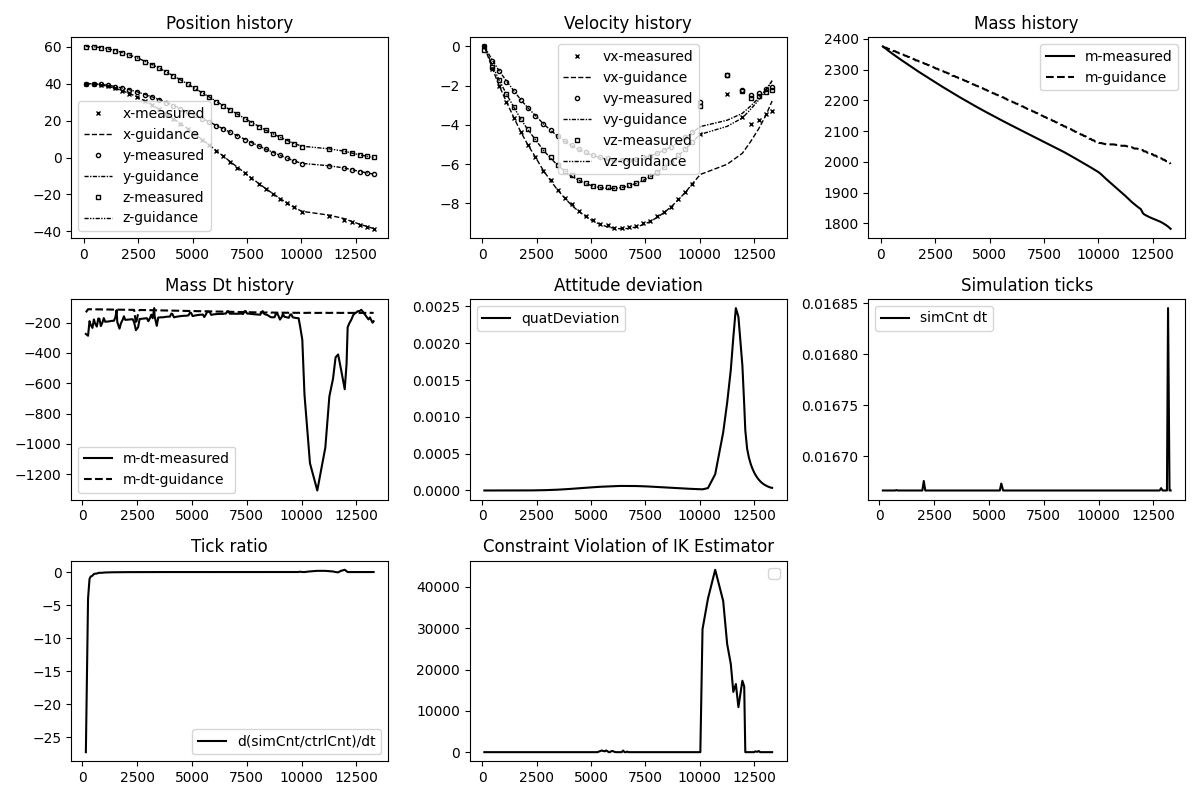
\includegraphics[width=1.0\linewidth]{is1_ep15}
     \vspace*{2mm}
     \caption{Episode 15 of $1^{st}$ input set}
     \label{fig:is1_ep15}
   \end{minipage}
\end{figure}

\begin{figure}[!htb]   
   \begin{minipage}{0.95\textwidth}
     \centering
     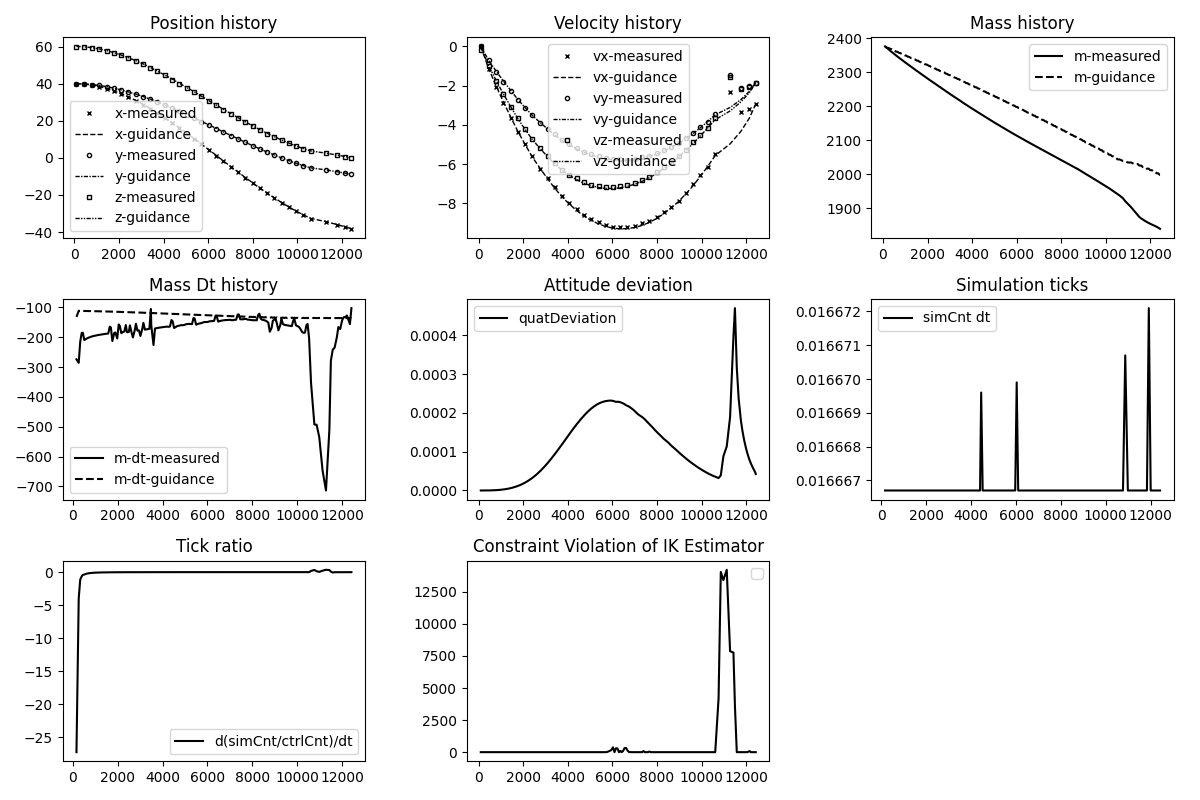
\includegraphics[width=1.0\linewidth]{is5_ep02}
     \vspace*{2mm}
     \caption{Episode 2 of $5^{th}$ input set}
     \label{fig:is5_ep02}
   \end{minipage}
\end{figure}

\begin{figure}[!htb]   
   \begin{minipage}{0.95\textwidth}
     \centering
     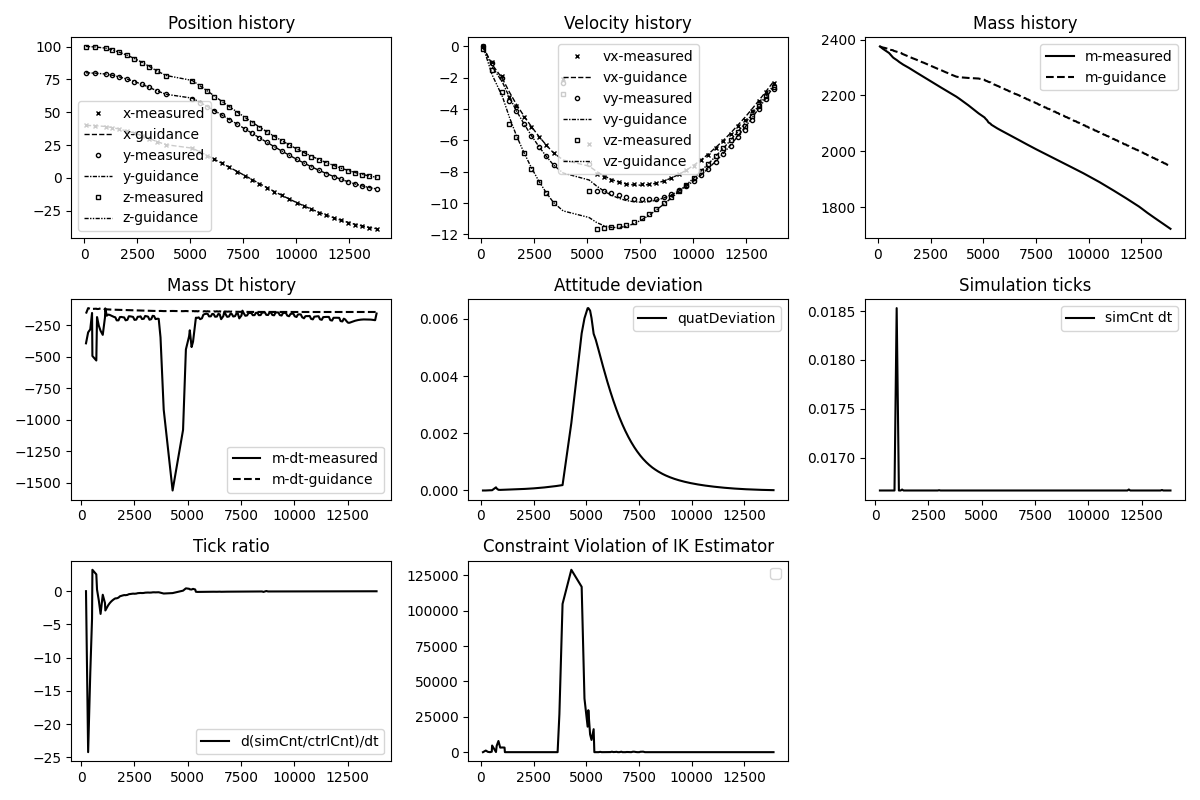
\includegraphics[width=1.0\linewidth]{is6_ep04}
     \vspace*{2mm}
     \caption{Episode 4 of $6^{th}$ input set}
     \label{fig:is6_ep04}
   \end{minipage}
\end{figure}

\section{Conclusion}
The guided path can be tracked closely by proposed controller(\cref{sec:controllerdesign}) regardless of that the rotational dynamics and disturbances(\cref{sec:disturbance}) are not accounted in \cref{sec:gdp}. The approach here is deterministic, capable of not only landing the plant but also imposing practical constraints such as descending speed, gliding cone region etc. on the path.  

In reality, engine thrust throttling capability is usually limited, i.e. with extra propellant loss when re-ignited or not re-ignitable, or could only reach certain values in $[\rho_1, \rho_2]$ \cite{casiano2010liquid,betts2010historical}, thus further development of the approach should take re-ignition cost and limitations, as well as discrete thrust throttling levels into account. Controllable fins and gimbaled thrusters can be considered to mitigate control difficulty introduced by limited thrust throttling capability, which could be included in further development in \cref{sec:controllerdesign} to take the non-linear dynamics and wind disturbance into account.    

\bibliographystyle{elsarticle-num}
\bibliography{citations.bib} 

\end{document}
